\textbf{\underline{OZ 3 - De Lorentzkracht en de wet van Ampère - Oefening 1:}}
\vspace{0.5cm}

Bereken de kracht die inwerkt op een oneindig lange, rechte draad met stroom $I$ ten gevolge van:
\begin{enumerate}[(a)]
    \item de vierkante spoel
    \item de driehoekige spoel
\end{enumerate}

\begin{center}
    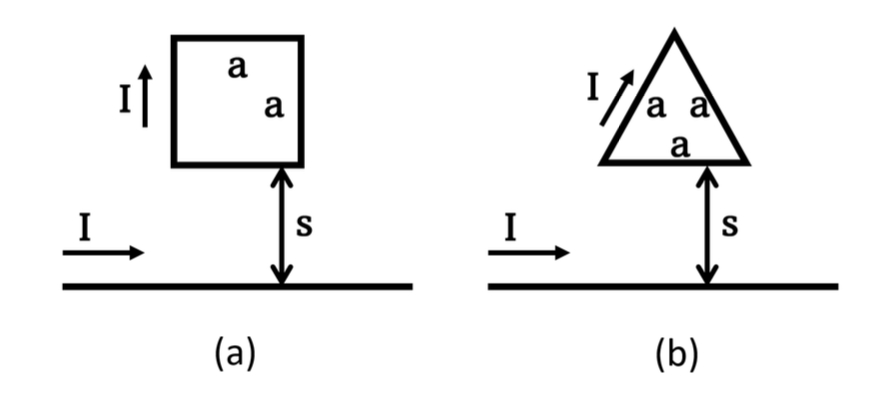
\includegraphics[scale = 0.5]{oz03/resources/Oz3Oef1.png}
\end{center}

% \begin{description}[labelwidth=1.5cm, leftmargin=!]
%     \item[Geg. :]   
%     \item[Gevr. :]  
%     \item[Opl. :]  
% \end{description}

\begin{enumerate}[(a)]
    \item 
        \begin{description}[labelwidth=1.5cm, leftmargin=!]
            \item[Geg. :]   $I$,$s$,$a$
            \item[Gevr. :]  de lorentzkracht $F_L$
            \item[Opl. :]   De evenwijdige zijden zullen een kracht uitoefenen op de draad. We vinden: 
                            \begin{align*}
                                \vec{F}_L &= \vec{F}_{\parallel, s+a} - \vec{F}_{\parallel, s}\\ 
                                    &= \dfrac{\mu_0I^2a}{2\pi}\left( \dfrac{1}{s} - \dfrac{1}{s+a} \right) \ (\hat{j}) \\
                                    &= \dfrac{\mu_0I^2}{2\pi}\dfrac{a^2}{s(s+a)} \ (\hat{j})
                            \end{align*}
        \end{description}
    \item 
        \begin{description}[labelwidth=1.5cm, leftmargin=!]
            \item[Geg. :]   $I$,$s$,$a$
            \item[Gevr. :]  de lorentzkracht $F_L$
            \item[Opl. :]                              
                        Een infinitesimale stukje $d\vec{\ell}$ van de linkse en rechtse schuine zijden kunnen we vectorieel voorstellen als
                        \begin{equation*}
                            d\vec{\ell}_l = dl\left(\cos(60^\circ) \hat{i} + \sin(60^\circ) \hat{j} \right), \ d\vec{\ell}_r = dl\left(\cos(60^\circ) \hat{i} - \sin(60^\circ) \hat{j} \right).
                        \end{equation*}
                        Als we over de hele schuine zijde $\ell$ integreren, dan heffen de verticale componenten elkaar op en blijft enkel de horizontale component over. We vinden:
                        \begin{align*}
                            \vec{F}_{\text{l+r}} 
                                &= \int Id\vec{\ell} \times \vec{B} \\ 
                                &= \frac{\mu_0I^2}{2\pi} \int \frac{1}{r} d\ell \ (-\hat{j}) \\
                                % &= \frac{\mu_0I^2}{2\pi} \int_0^a \frac{1}{r} d\ell_L \ (\hat{j}) \\
                                &= \frac{\mu_0I^2}{\pi} \int_0^a \frac{1}{r} \cos(60^\circ)d\ell \ (-\hat{j}) \\
                                &= \frac{\mu_0I^2}{\pi} \frac{\cos(60^\circ)}{\sin(60^\circ)} \int_{s}^{s+a\sin(60^\circ)} \frac{1}{r} dr \ (-\hat{j}) \\
                                &= \frac{\mu_0I^2}{2\pi} \frac{1}{\sin(60^\circ)} \ln\left(\frac{s+a\sin(60^\circ)}{s}\right) \ (-\hat{j})
                        \end{align*}
                        Als we $\vec{F}_{\parallel, s}$ hernemen uit (a), dan vinden we voor de totale kracht van heel de driehoek:
                        \begin{equation*}
                            \vec{F}_L = \vec{F}_{\text{l+r}} + \vec{F}_{\parallel, s} = \frac{\mu_0I^2}{2\pi}\left(\frac{a}{s} - \frac{1}{\sin(60^\circ)}\ln\left(\frac{s+a\sin(60^\circ)}{s}\right)\right)  \ (\hat{j})
                        \end{equation*}
        \end{description}
        
\end{enumerate}

\vspace{1cm}